\documentclass{article}
\usepackage{amsmath}
\usepackage{amsthm}
\usepackage{graphicx,subfigure}
\usepackage{url,color}
\usepackage[colorlinks=true, linkcolor=blue, urlcolor=blue, citecolor=blue, pdfborder={0 0 1}]{hyperref}
\title{CIS 579 Fall 2024 Programming Assignment 1}
\author{Due 10/14/2024 11:59 pm, Total:[160 marks]}
\date{}
\begin{document}
\maketitle

\noindent Please submit everything through Canvas.\\
\section{Problems}
\noindent a) In this programming assignment, you will solve the 8-Puzzle Problem. The 8-Puzzle problem consists of a (3*3) grid with one blank space and eight numbered tiles. The goal is to arrange the tiles in numerical order by sliding them into the empty space. The action space can be thought of as the blank tile moving UP, DOWN, LEFT and RIGHT. You can consider path cost to be +1 for every tile moved. A sample initial and goal configuration looks like this:\\

\begin{figure}[ht]
    \centering
    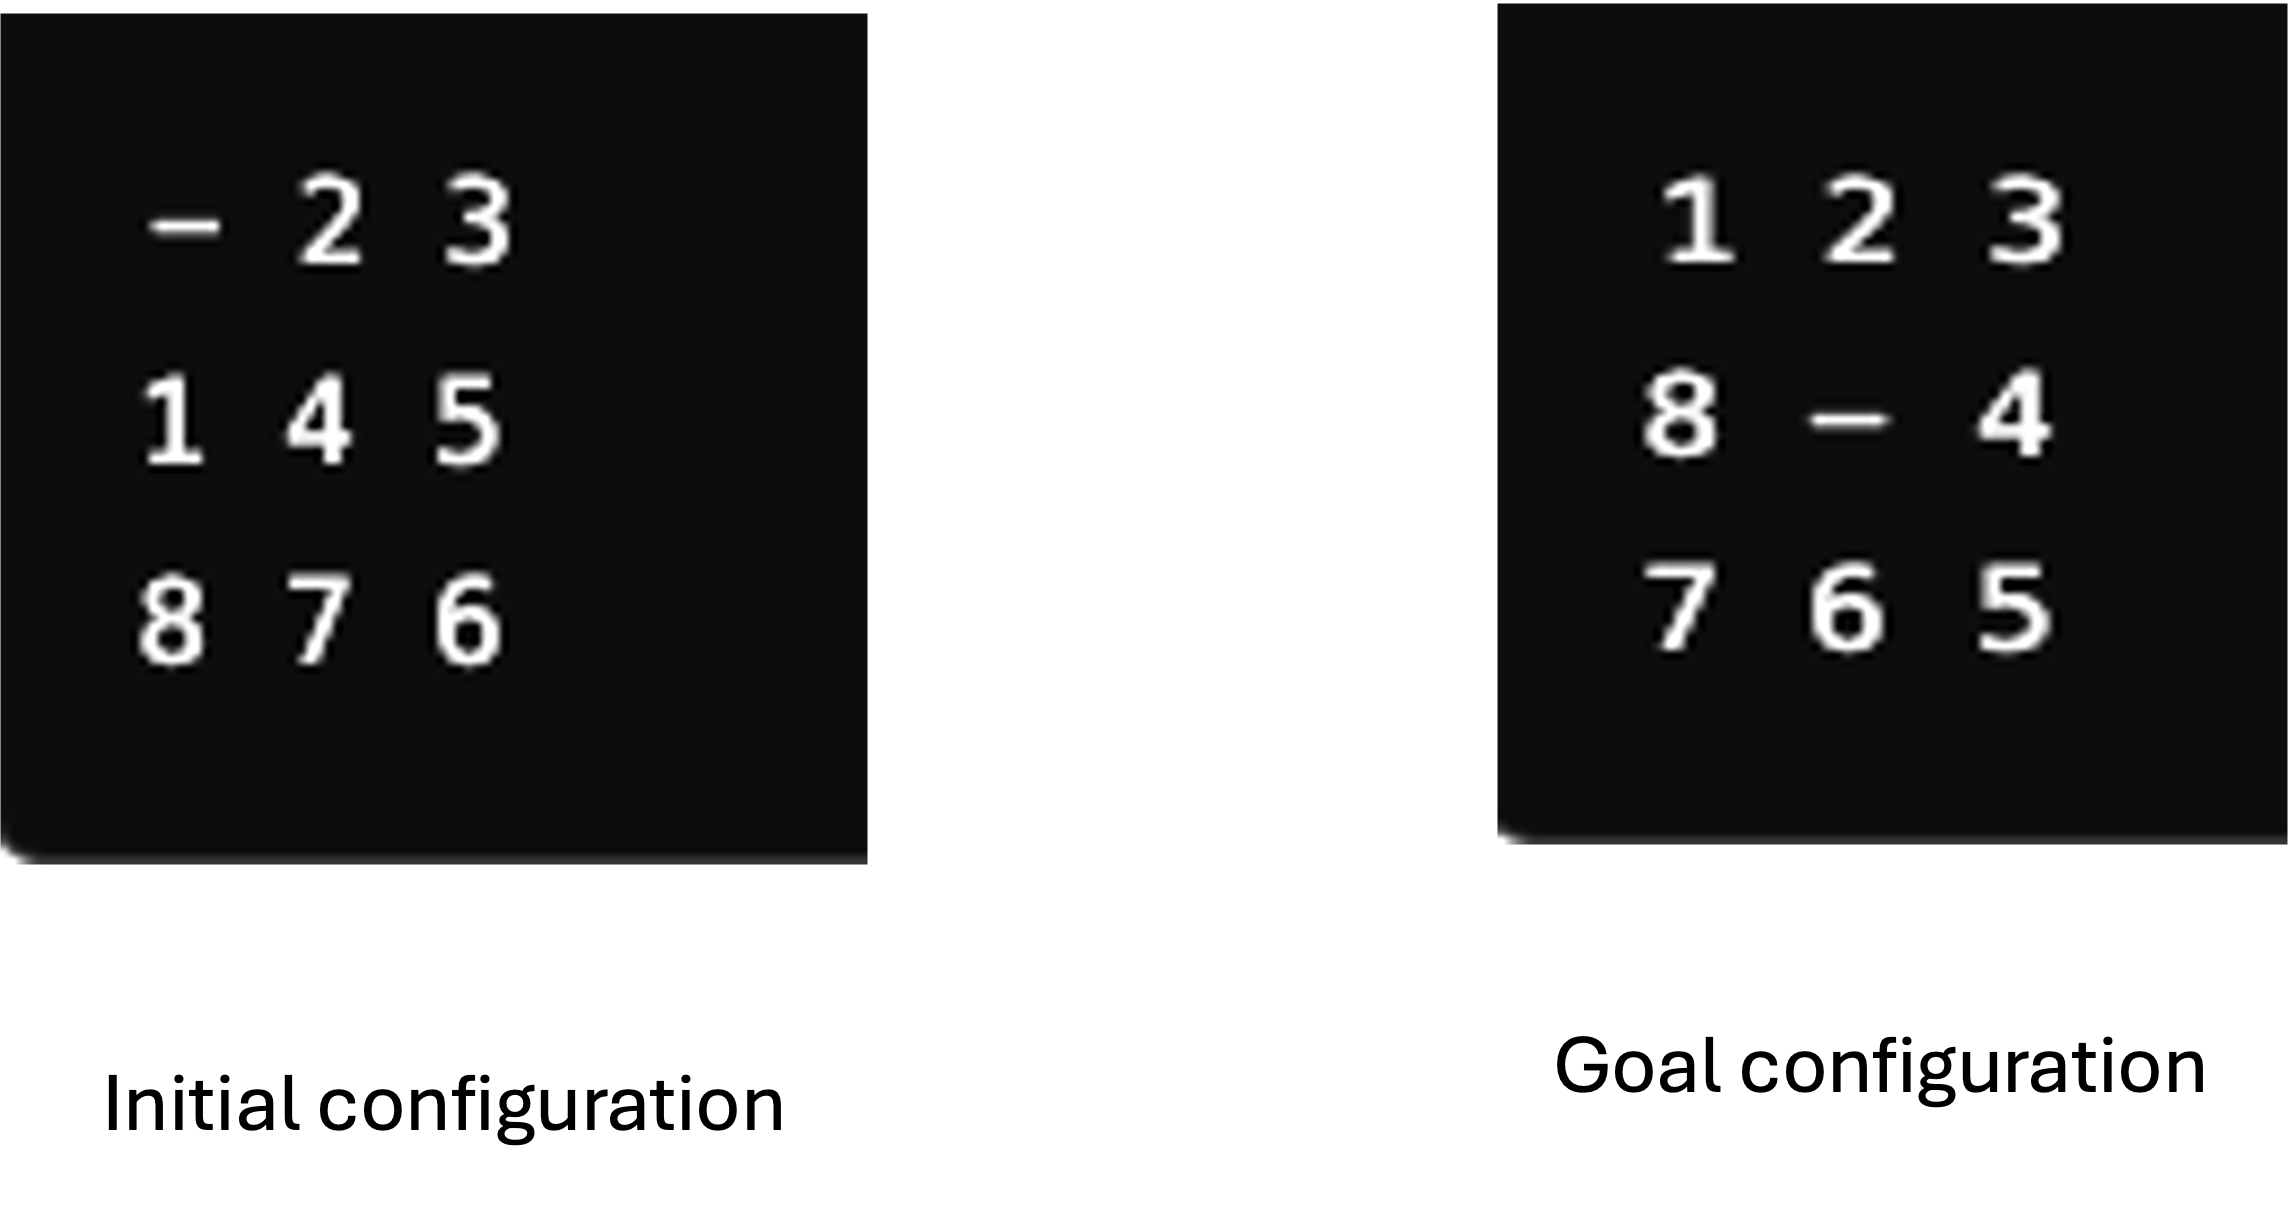
\includegraphics[width=0.5\linewidth]{Images/8-Queens.png}
    \caption{8-Puzzle Problem (initial and goal configuration}
    \label{fig:STate-space}
\end{figure}

\noindent For the above initial and goal configuration, implement the below search strategies:\\
\begin{enumerate}
    \item BFS Search [20 marks]
    \item DFS Search [20 marks]
    \item Uniform Cost Search [20 marks]
    \item Greedy Best First Search with heuristic functions as below\\
     a)\# of misplaced tiles [20 marks]\\
     b) Manhattan distance [20 marks] \\
     c) Any other heuristic you can think of? (This is optional)\\
     \item $A^{*}$ Search with heuristic functions as below\\
     a)\# of misplaced tiles [20 marks] \\
     b) Manhattan distance  [20 marks]\\
     c) Any other heuristic you can think of? (This is optional)\\
\end{enumerate}

\noindent Please have a single code (eightpuzzle.py) which triggers all the above-mentioned search functions. All the search functions can be in a different python code (however not a strict requirement).The command line input to test your code will be as below:\\

\noindent python eightpuzzle.py --search ``DFS/BFS/UCS/GBS/A*" --initial `[[-,2,3],[1,4,5],[8,7,6]]' --goal `[[1,2,3],[8,-,4],[7,6,5]]' --heuristic ``misplaced/manhattan/other".\\

\noindent \textbf{Your code should output} the following details for each search algorithm, please generate the search output in a different text file named \textbf{output\_\{search\}\_\{heuristic\}.txt} for each search algorithm. Below is the naming convention:
\begin{enumerate}
\item DFS: output\_DFS.txt

\item BFS: output\_BFS.txt

\item UCS, misplaced heuristic : output\_UCS.txt

\item GBS, misplaced heuristic : output\_GBS\_misplaced.txt

\item GBS, manhattan heuristic : output\_GBS\_manhattan.txt

\item GBS, other heuristic : output\_GBS\_other.txt (optional)

\item A*, misplaced heuristic: output\_A*\_misplaced.txt

\item A*, manhattan heuristic : output\_A*\_manhattan.txt

\item A*, other heuristic : output\_A*\_other.txt (optional)
\end{enumerate}
Your search output in these files should contain the following details:
\begin{enumerate}
    \item  Path: This should output the entire search path (states and actions). You could either output the states as a board or as a 2D list as in command line. Please output the path as: $(s_1,a_1)->(s_2,a_2)->.....->(s_g) $ where $s_1$ is the initial state and $s_g$ is the goal state. You can print these sequences out as strings in the output file. Please enter a header (BFS/DFS/UCS/GBS,$A^*$) for every search algorithm followed by a ``**********" before printing out the paths.
    \item Path cost
    \item Depth of the Search Tree
    \item Time taken to run the specific algorithm
    \item  Number of nodes expanded by the search tree (memory usage)
\end{enumerate}


\noindent b) At the end, create a table comparing these various outputs of your implementation for all the different search algorithms (with all the heuristics). [20 marks]\\

\section {Deliverables}
\begin{enumerate}
    \item Code along with proper read me document. The folder should contain a eightpuzzle.py code which takes in the relevant command line parameters.
    \item Output file: output.txt with the outputs of the various search algorithms (search output, path cost, depth, time and number of expanded nodes). For submission, you can either append all the output to a single output.txt file or keep different output files for different search algorithms. 
    \item A pdf file containing a table with the algorithms as columns and path-cost, depth, time taken and number of expanded nodes as rows. If you have any interesting heuristic that you used for Informed Search (this is optional), please also describe them in detail in this document.
\end{enumerate}

\section {Resources}
\begin{enumerate}
    \item  Consider using libraries like heapq for priority queues or collections.deque for queues.
    \item Review lecture materials and the book for search algorithms.
    \item You can also ballpark your solutions using the software: \href{https://tristanpenman.com/demos/n-puzzle/}{https://tristanpenman.com/demos/n-puzzle/} to get an idea.
    \item I am attaching a small filler template code which you might find helpful and use it while writing your code. The file ``eightpuzzle.py" is the main file that will trigger the search. You have to modify this code as required by taking in command line arguments and also produce the required output for the assignment. Remember, this is not a complete runnable code. It calls ``search.py" which consists of a general search problem template that you can fill in. It has predefined functions for BFS, DFS, etc where you can write your code.  The code template is taken from The Pacman AI projects developed at UC Berkeley, \href{http://ai.berkeley.edu}{http://ai.berkeley.edu}
%{https://tristanpenman.com/demos/n-puzzle/}
\end{enumerate}
% Consider using libraries like heapq for priority queues or collections.deque for queues.
% Review lecture materials and the book for search algorithms. You can also ballpark your solutions using the software: \href{https://tristanpenman.com/demos/n-puzzle/} {https://tristanpenman.com/demos/n-puzzle/} to get an idea.
% %{https://tristanpenman.com/demos/n-puzzle/}

%\noindent c)

% \begin{enumerate}

% %\item \textbf{Question 1.7} 

% \item \textbf{Question 2.4} [10 marks]

% \item \textbf{Question 2.7} [20 marks]


% \item \textbf{Question 2.10} [20 marks]

% \item \textbf{Question 2.13, part a.} [10 marks]
% %\item \textbf{Question 3.9 a \& c}. Ignore part b as it involves implementation
% \item \textbf{Question 3.8} [20 marks]
% \item \textbf{Question 3.9, part a and c} [20 marks]

% \end{enumerate}




\end{document}
